\section{Evaluation}
\label{sec:eval}
We ask: is unsoundness pervasive (RQ1); does priced-receipt clearing beat a sound over-approximation, and does the guarantee hold (RQ2); how do pricers compare, and does the key matter (RQ3); how good is the key behind the clearances (RQ4); how faithful is our analysis to FlowDroid (RQ5); what does it cost (RQ6); do the validity checks hold up (RQ7); which design choices matter (RQ8); does the pricer hold up on code it knows less well (RQ9); and does it matter for real leaks (RQ10).

\subsection{RQ1: Is unsoundness pervasive?}
\label{sec:rq1}
Of the 17{,}830 framework methods on source-to-sink paths, 12{,}274 are not modeled by FlowDroid.
We ran FlowDroid on 40 random small apps with and without its library summaries (\texttt{-tw NONE}).
In the 29 apps where neither run was cut short, FlowDroid reports 20 leaking sink methods with summaries and 2 without; over 36 apps 54 of 63 (86\%) leaks vanish, and none appears only without the summaries (Table~\ref{tab:fd-none}).
This is the extreme case: it measures how much a library model matters, not what FlowDroid misses with its default summaries.
\tabph{4.4cm}{tab:fd-none}{FlowDroid with and without its library summaries on the same apps.}{Per-app table or summary rows: leaking sink methods with summaries, without, only-with, only-without; complete versus partial runs. \textbf{Have} for 40 apps (36 with both answers); \textbf{scheduled}: 40 more apps to reach 80 (tighter interval).}

\subsection{RQ2: Does it clear more than a sound analysis, and does the guarantee hold?}
\label{sec:rq2}
A sound over-approximation (every hole is a flow) clears 72.0\% of the 101{,}090 leak-free sinks with a non-constant argument; the remaining 28.0\% are the hard slice.
Table~\ref{tab:main} shows what priced receipts clear of it, and Figure~\ref{fig:curve} the whole trade-off.
\begin{table}[t]
\caption{Main key, 324 apps. Share of the 28{,}335 clean hole-dependent verdicts cleared, and held-out apps with a wrong clearance (in brackets), by target $\alpha$.}
\label{tab:main}
\small
\begin{tabular}{@{}lccc@{}}
\toprule
Pricer & $\alpha{=}0.10$ & $\alpha{=}0.05$ & $\alpha{=}0.02$\\
\midrule
Counting (flat price) & 0\% & 0\% & --\\
Frequency prior & 9.2\% (4.9\%) & 6.6\% (0.8\%) & --\\
Feature classifier & 33.2\% (5.4\%) & 22.0\% (0.7\%) & --\\
Sonnet~5 probabilities & 53.0\% (5.6\%) & 29.6\% (2.5\%) & --\\
Jev & 40.0\% (1.0\%) & 40.0\% (1.0\%) & 33.4\% (0.3\%)\\
\bottomrule
\end{tabular}
\end{table}
\begin{figure}[t]
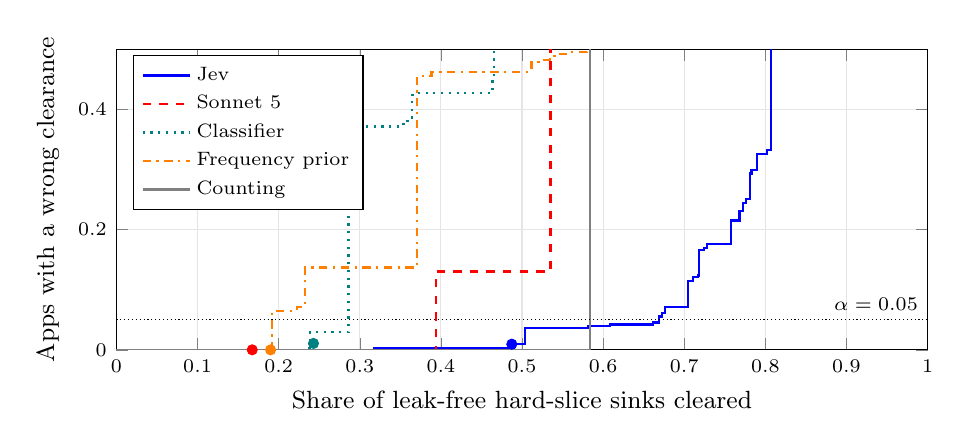
\begin{tikzpicture}
\begin{axis}[width=0.98\linewidth, height=5.4cm, xmin=0, xmax=1, ymin=0, ymax=0.5,
  xlabel={Share of leak-free hard-slice sinks cleared}, ylabel={Apps with a wrong clearance},
  legend style={font=\scriptsize, at={(0.02,0.98)}, anchor=north west}, legend cell align=left,
  tick label style={font=\scriptsize}, label style={font=\small}, grid=major, grid style={gray!20}]
\addplot[blue, thick, const plot mark left] coordinates {(0.0002,0.0000) (0.0605,0.0000) (0.0827,0.0000) (0.0921,0.0000) (0.1181,0.0000) (0.1841,0.0000) (0.1897,0.0000) (0.1965,0.0000) (0.2407,0.0000) (0.2520,0.0000) (0.2762,0.0000) (0.2994,0.0000) (0.3050,0.0000) (0.3118,0.0000) (0.3180,0.0033) (0.3261,0.0033) (0.3355,0.0033) (0.3520,0.0033) (0.3597,0.0033) (0.3755,0.0033) (0.4735,0.0033) (0.4902,0.0098) (0.5009,0.0098) (0.5032,0.0358) (0.5102,0.0358) (0.5233,0.0358) (0.5820,0.0391) (0.5871,0.0391) (0.5936,0.0391) (0.6010,0.0391) (0.6087,0.0423) (0.6149,0.0423) (0.6450,0.0423) (0.6527,0.0423) (0.6610,0.0456) (0.6685,0.0554) (0.6721,0.0619) (0.6760,0.0717) (0.7044,0.1140) (0.7110,0.1205) (0.7170,0.1238) (0.7185,0.1661) (0.7241,0.1694) (0.7285,0.1759) (0.7580,0.2150) (0.7666,0.2150) (0.7680,0.2313) (0.7728,0.2443) (0.7760,0.2508) (0.7802,0.2508) (0.7807,0.2932) (0.7830,0.2997) (0.7900,0.3257) (0.7994,0.3257) (0.8018,0.3322) (0.8065,0.8208) (0.8082,0.8274) (0.8133,0.8339) (0.8182,0.8339) (0.8347,0.8371) (0.8394,0.8534) (0.8469,0.8567) (0.8750,0.8567) (0.8798,0.8632) (0.8821,0.8697) (0.8847,0.8762) (0.8917,0.8827) (0.9022,0.8860) (0.9205,0.8860) (0.9270,0.8860) (0.9336,0.8860) (0.9522,0.8860) (0.9590,0.8860) (0.9665,0.8860) (0.9716,0.8860) (0.9774,0.8860) (0.9831,0.8893) (0.9878,0.8925) (0.9919,0.8958) (0.9955,0.9251) (1.0000,0.9349)};
\addlegendentry{Jev}
\addplot[red, thick, dashed, const plot mark left] coordinates {(0.0000,0.0000) (0.1674,0.0000) (0.3939,0.1303) (0.4285,0.1303) (0.5350,0.8078) (0.5918,0.8111) (0.6068,0.8111) (0.6350,0.8111) (0.6608,0.8111) (0.6805,0.8111) (0.6948,0.8404) (0.7063,0.8404) (0.7202,0.8436) (0.7305,0.8436) (0.7356,0.8436) (0.7433,0.8436) (0.8195,0.8436) (0.8274,0.8436) (0.8509,0.8436) (0.8554,0.8436) (0.8637,0.8436) (0.8687,0.8469) (0.8772,0.8469) (0.8823,0.8469) (0.9109,0.8469) (0.9184,0.8469) (0.9287,0.8534) (0.9332,0.8534) (0.9383,0.8534) (0.9545,0.8534) (0.9616,0.8567) (0.9902,0.8567) (0.9910,0.8664) (0.9987,0.8827) (0.9998,0.8925) (1.0000,0.9349)};
\addlegendentry{Sonnet~5}
\addplot[teal, thick, dotted, const plot mark left] coordinates {(0.0000,0.0000) (0.2307,0.0000) (0.2351,0.0033) (0.2382,0.0293) (0.2804,0.0293) (0.2862,0.0293) (0.2862,0.3648) (0.2879,0.3713) (0.3539,0.3811) (0.3637,0.3811) (0.3646,0.4235) (0.3693,0.4267) (0.3750,0.4267) (0.4184,0.4267) (0.4635,0.4528) (0.4650,0.5342) (0.4710,0.5342) (0.4754,0.5342) (0.4757,0.5440) (0.4819,0.5440) (0.5784,0.5472) (0.5829,0.5472) (0.5867,0.5570) (0.5920,0.5570) (0.6002,0.5668) (0.6049,0.5668) (0.6166,0.5668) (0.6190,0.5831) (0.6205,0.6026) (0.6252,0.6091) (0.6329,0.6091) (0.6401,0.6091) (0.6454,0.6091) (0.6516,0.6124) (0.7302,0.6124) (0.7382,0.6124) (0.7439,0.6124) (0.7456,0.6319) (0.7591,0.6352) (0.7649,0.6515) (0.7713,0.6515) (0.7806,0.6515) (0.7868,0.6515) (0.7909,0.6547) (0.8012,0.6547) (0.8041,0.6678) (0.8063,0.6808) (0.8084,0.7948) (0.8125,0.7948) (0.8197,0.7948) (0.8261,0.7980) (0.8304,0.8436) (0.8349,0.8436) (0.8413,0.8436) (0.8481,0.8436) (0.8541,0.8436) (0.8595,0.8502) (0.8637,0.8502) (0.8695,0.8502) (0.8744,0.8502) (0.8751,0.8599) (0.8825,0.8664) (0.8939,0.8664) (0.9022,0.8697) (0.9077,0.8697) (0.9107,0.8795) (0.9124,0.9023) (0.9259,0.9055) (0.9304,0.9088) (0.9387,0.9088) (0.9622,0.9088) (0.9667,0.9186) (0.9964,0.9186) (0.9977,0.9251) (1.0000,0.9349)};
\addlegendentry{Classifier}
\addplot[orange, thick, dashdotted, const plot mark left] coordinates {(0.0053,0.0000) (0.0651,0.0000) (0.0696,0.0000) (0.0754,0.0000) (0.1140,0.0000) (0.1841,0.0000) (0.1897,0.0000) (0.1922,0.0651) (0.2131,0.0651) (0.2228,0.0717) (0.2319,0.0717) (0.2320,0.1368) (0.3706,0.4560) (0.3795,0.4560) (0.3883,0.4625) (0.4882,0.4625) (0.5105,0.4625) (0.5109,0.4691) (0.5117,0.4788) (0.5220,0.4788) (0.5269,0.4821) (0.5342,0.4886) (0.5401,0.4919) (0.5476,0.4919) (0.5560,0.4951) (0.5799,0.5179) (0.5848,0.5179) (0.6408,0.5212) (0.6470,0.5212) (0.6502,0.5342) (0.6506,0.5407) (0.6566,0.5407) (0.6615,0.5440) (0.6642,0.6026) (0.6707,0.6026) (0.6794,0.6156) (0.6929,0.6156) (0.7021,0.6254) (0.7161,0.6254) (0.7194,0.6450) (0.7226,0.6580) (0.7268,0.6612) (0.7279,0.6678) (0.7381,0.6710) (0.7420,0.6775) (0.7488,0.7068) (0.7529,0.7068) (0.7563,0.7166) (0.7580,0.7655) (0.7621,0.7687) (0.7681,0.7785) (0.7736,0.7818) (0.7830,0.7915) (0.7901,0.8697) (0.7943,0.9088) (0.8409,0.9088) (0.8490,0.9088) (0.8556,0.9121) (0.8599,0.9121) (0.8881,0.9121) (0.8968,0.9121) (0.9011,0.9121) (0.9062,0.9186) (0.9127,0.9186) (0.9133,0.9251) (0.9186,0.9251) (0.9285,0.9251) (0.9383,0.9251) (0.9466,0.9251) (0.9603,0.9251) (0.9663,0.9283) (0.9712,0.9283) (0.9795,0.9283) (0.9846,0.9283) (0.9866,0.9349) (0.9919,0.9349) (0.9996,0.9349)};
\addlegendentry{Frequency prior}
\addplot[gray, thick, const plot mark left] coordinates {(0.0000,0.0000) (0.5835,0.8664) (0.7390,0.8860) (0.8466,0.8893) (0.8862,0.9283) (0.9041,0.9349) (0.9297,0.9349) (0.9440,0.9349) (0.9502,0.9349) (0.9720,0.9349) (0.9780,0.9349) (0.9851,0.9349) (0.9915,0.9349) (0.9968,0.9349)};
\addlegendentry{Counting}
\addplot[only marks, mark=*, mark size=1.8pt, blue, forget plot] coordinates {(0.4874,0.0094)};
\addplot[only marks, mark=*, mark size=1.8pt, red, forget plot] coordinates {(0.1674,0.0000)};
\addplot[only marks, mark=*, mark size=1.8pt, teal, forget plot] coordinates {(0.2429,0.0107)};
\addplot[only marks, mark=*, mark size=1.8pt, orange, forget plot] coordinates {(0.1900,0.0000)};
\addplot[black, densely dotted, forget plot] coordinates {(0,0.05) (1,0.05)};
\node[font=\scriptsize, anchor=south east] at (axis cs:1,0.05) {$\alpha=0.05$};
\end{axis}
\end{tikzpicture}

\caption{Risk against coverage on all 324 apps (main key) as the threshold grows. Dots: mean certified operating point at $\alpha=0.05$ over 200 half splits. Counting stays on the vertical axis: any threshold that clears something puts a wrong clearance in most apps.}
\label{fig:curve}
\end{figure}
At the certified thresholds, receipts clear 40\% of the hard slice at $\alpha=0.05$ with 1.0\% of held-out apps wrong; with the sound part, 83.2\% of all leak-free sinks against 72.0\%.
The observed error stays below $\alpha$ for every pricer, as the theory predicts, while the power differs by a factor of six (0\% to 40\% at $\alpha=0.05$).
Counting the assumptions is unsafe even at one fact: clearing every receipt of size one gives a wrong clearance in 93\% of the apps.
The three wrong clearances at the chosen threshold come from three different facts and apps, not from one widely bundled fact (Figure~\ref{fig:receipt}).

\subsection{RQ3: How do pricers compare, and does the key matter?}
\label{sec:rq3}
Table~\ref{tab:keys} repeats the main pricers under the other keys, and Figure~\ref{fig:deletion} shows the deletion benchmark as more classes are removed.
\begin{table}[t]
\caption{Other keys. Share cleared at $\alpha=0.05$ (held-out apps with a wrong clearance). Deletion: whole classes removed, 3 seeds.}
\label{tab:keys}
\small
\begin{tabular}{@{}lcccc@{}}
\toprule
Key & Jev & Sonnet~5 & Classifier & LLM as fact\\
\midrule
Audited (324 apps) & 39.4\% (2.0\%) & -- & -- & --\\
K2, code-derived (322 apps) & 25.7\% (1.7\%) & 33.6\% (2.3\%) & 20.4\% (2.3\%) & 38.5\% (2.5\%)\\
Deletion, 25\% of classes & 52.2\% (0.8\%) & 81.9\% (0.5\%) & 71.4\% (1.6\%) & 79.8\% (1.2\%)\\
Deletion, 75\% of classes & 50.9\% (1.3\%) & 79.1\% (1.0\%) & 33.1\% (0.5\%) & --\\
\bottomrule
\end{tabular}
\end{table}
\begin{figure}[t]
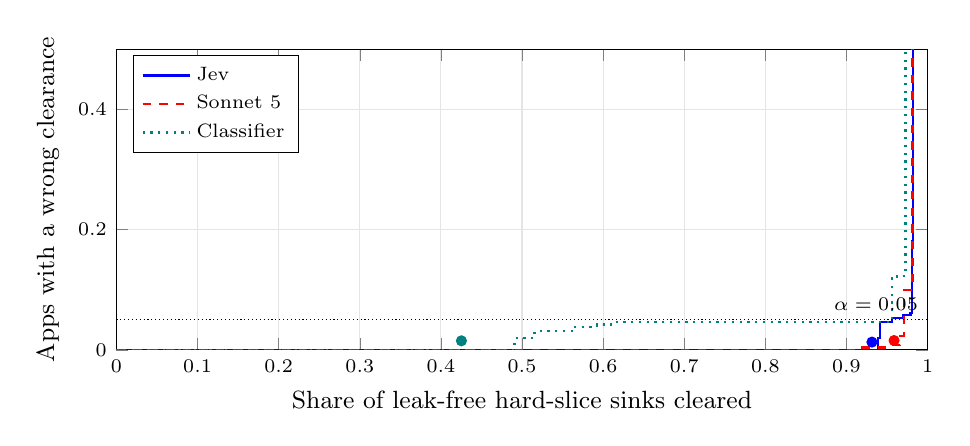
\begin{tikzpicture}
\begin{axis}[width=0.98\linewidth, height=5.4cm, xmin=0, xmax=1, ymin=0, ymax=0.5,
  xlabel={Share of leak-free hard-slice sinks cleared}, ylabel={Apps with a wrong clearance},
  legend style={font=\scriptsize, at={(0.02,0.98)}, anchor=north west}, legend cell align=left,
  tick label style={font=\scriptsize}, label style={font=\small}, grid=major, grid style={gray!20}]
\addplot[blue, thick, const plot mark left] coordinates {(0.0008,0.0000) (0.2407,0.0000) (0.3207,0.0000) (0.4006,0.0000) (0.4068,0.0000) (0.4208,0.0000) (0.4332,0.0000) (0.4387,0.0000) (0.4457,0.0000) (0.4519,0.0000) (0.4674,0.0000) (0.4759,0.0000) (0.8634,0.0000) (0.8960,0.0000) (0.9006,0.0000) (0.9154,0.0000) (0.9216,0.0000) (0.9262,0.0000) (0.9332,0.0000) (0.9387,0.0000) (0.9387,0.0192) (0.9410,0.0345) (0.9410,0.0460) (0.9457,0.0460) (0.9534,0.0460) (0.9565,0.0536) (0.9643,0.0536) (0.9697,0.0575) (0.9790,0.0613) (0.9806,0.0881) (0.9806,0.0958) (0.9806,0.1111) (0.9806,0.1801) (0.9821,0.6552) (0.9845,0.6667) (0.9845,0.6935) (0.9891,0.6973) (0.9899,0.7280) (0.9946,0.7318) (0.9953,0.7548) (0.9961,0.8506) (1.0000,0.8582) (1.0000,0.8736) (1.0000,0.8889)};
\addlegendentry{Jev}
\addplot[red, thick, dashed, const plot mark left] coordinates {(0.0000,0.0000) (0.3106,0.0000) (0.8393,0.0000) (0.8804,0.0000) (0.8859,0.0000) (0.9053,0.0000) (0.9177,0.0038) (0.9332,0.0038) (0.9464,0.0038) (0.9534,0.0077) (0.9581,0.0077) (0.9635,0.0077) (0.9658,0.0230) (0.9713,0.0920) (0.9713,0.0996) (0.9814,0.6169) (0.9821,0.6284) (0.9837,0.6360) (0.9884,0.6398) (0.9884,0.6782) (0.9884,0.7011) (0.9884,0.7165) (0.9907,0.7318) (0.9946,0.7395) (0.9946,0.8544) (0.9961,0.8621) (0.9992,0.8697) (1.0000,0.8889)};
\addlegendentry{Sonnet~5}
\addplot[teal, thick, dotted, const plot mark left] coordinates {(0.0000,0.0000) (0.3781,0.0000) (0.3913,0.0000) (0.3991,0.0000) (0.4907,0.0192) (0.4969,0.0192) (0.5155,0.0307) (0.5202,0.0307) (0.5303,0.0307) (0.5357,0.0307) (0.5637,0.0383) (0.5815,0.0383) (0.5924,0.0421) (0.5994,0.0421) (0.6095,0.0460) (0.9301,0.0460) (0.9356,0.0460) (0.9402,0.0460) (0.9449,0.0460) (0.9503,0.0460) (0.9557,0.0460) (0.9557,0.1188) (0.9620,0.1226) (0.9666,0.1226) (0.9728,0.1226) (0.9728,0.5441) (0.9728,0.5594) (0.9728,0.5670) (0.9736,0.6092) (0.9736,0.6322) (0.9736,0.6398) (0.9845,0.6398) (0.9891,0.6475) (0.9899,0.8314) (0.9899,0.8391) (0.9922,0.8467) (0.9969,0.8506) (0.9992,0.8659) (1.0000,0.8736) (1.0000,0.8889)};
\addlegendentry{Classifier}
\addplot[only marks, mark=*, mark size=1.8pt, blue, forget plot] coordinates {(0.9314,0.0129)};
\addplot[only marks, mark=*, mark size=1.8pt, red, forget plot] coordinates {(0.9587,0.0155)};
\addplot[only marks, mark=*, mark size=1.8pt, teal, forget plot] coordinates {(0.4253,0.0150)};
\addplot[black, densely dotted, forget plot] coordinates {(0,0.05) (1,0.05)};
\node[font=\scriptsize, anchor=south east] at (axis cs:1,0.05) {$\alpha=0.05$};
\end{axis}
\end{tikzpicture}

\caption{Risk against coverage under the code-derived key K2 (322 apps). The language model's yes/no taken as fact is a single operating point (clear when the model says no to every receipt fact); priced pricers give a curve on which the risk can be chosen.}
\label{fig:curve-k2}
\end{figure}
The guarantee holds under every key (wrong clearances at most 2.5\%); the ranking of pricers does not. (Figure~\ref{fig:curve-k2})
The classifier is strong when single methods are deleted (82--88\%, because it learns FlowDroid's conventions from sibling methods) and collapses when whole classes are removed (33\% at 75\%), the realistic case, since 86\% of the unmodeled methods that matter sit in classes with no modeled method.
A general language model asked for probabilities is the best or tied pricer under K2 and on the deletion keys; Jev leads only on the main key at $\alpha=0.05$ and is about 40 times cheaper (about \$0.4 against \$16 for the corpus).
The model's yes/no taken as fact has no knob: it clears 38--90\% depending on the key, with wrong clearances in 0 to 8\% of apps and a risk that cannot be chosen.

\begin{figure}[t]
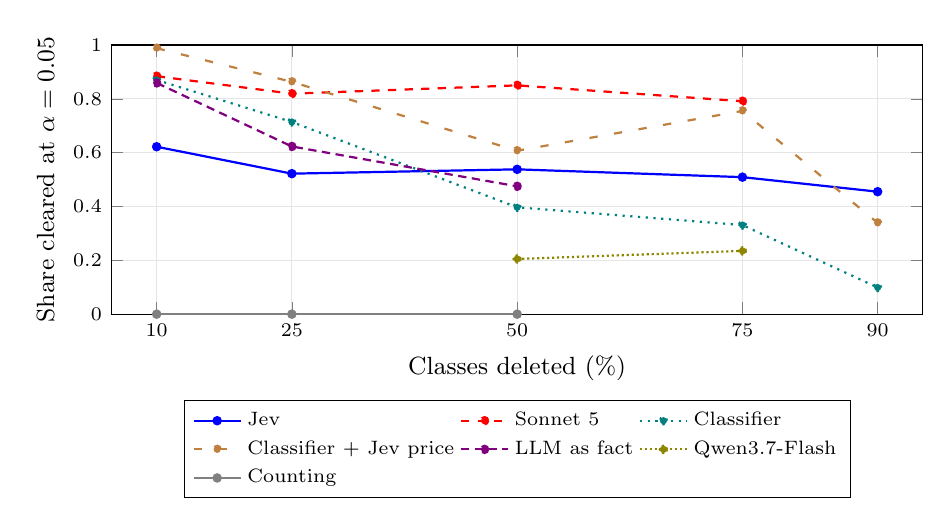
\begin{tikzpicture}
\begin{axis}[width=0.98\linewidth, height=5cm, xmin=5, xmax=95, ymin=0, ymax=1,
  xlabel={Classes deleted (\%)}, ylabel={Share cleared at $\alpha=0.05$}, xtick={10,25,50,75,90},
  legend style={font=\scriptsize, at={(0.5,-0.32)}, anchor=north}, legend cell align=left, legend columns=3,
  tick label style={font=\scriptsize}, label style={font=\small}, grid=major, grid style={gray!20}]
\addplot[blue, thick, mark=*, mark size=1.3pt] coordinates {(10,0.6220) (25,0.5220) (50,0.5380) (75,0.5090) (90,0.4550)};
\addlegendentry{Jev}
\addplot[red, thick, dashed, mark=*, mark size=1.3pt] coordinates {(10,0.8840) (25,0.8190) (50,0.8500) (75,0.7910)};
\addlegendentry{Sonnet~5}
\addplot[teal, thick, dotted, mark=*, mark size=1.3pt] coordinates {(10,0.8700) (25,0.7140) (50,0.3970) (75,0.3310) (90,0.0990)};
\addlegendentry{Classifier}
\addplot[brown, thick, loosely dashed, mark=*, mark size=1.3pt] coordinates {(10,0.9880) (25,0.8630) (50,0.6070) (75,0.7550) (90,0.3390)};
\addlegendentry{Classifier + Jev price}
\addplot[violet, thick, densely dashed, mark=*, mark size=1.3pt] coordinates {(10,0.8590) (25,0.6230) (50,0.4750)};
\addlegendentry{LLM as fact}
\addplot[olive, thick, densely dotted, mark=*, mark size=1.3pt] coordinates {(50,0.2050) (75,0.2350)};
\addlegendentry{Qwen3.7-Flash}
\addplot[gray, thick, mark=*, mark size=1.3pt] coordinates {(10,0.0000) (25,0.0000) (50,0.0000)};
\addlegendentry{Counting}
\end{axis}
\end{tikzpicture}

\caption{Whole-class deletion: share of the leak-free hard slice cleared at $\alpha=0.05$ against the share of FlowDroid-modeled classes deleted (mean over three seeds; one seed at 90\%). Held-out apps with a wrong clearance stay at or below 1.6\% in every cell.}
\label{fig:deletion}
\end{figure}

\begin{table}[t]
\caption{Ranking quality is not what certification rewards. AUROC of the bound (real flows against leak-free sinks, all verdicts), and the certified result over 200 half splits.}
\label{tab:rank}
\small
\begin{tabular}{@{}llrrrr@{}}
\toprule
Key & Pricer & AUROC & Cleared, $\alpha{=}0.05$ & Wrong, mean / p95 & Cleared, $\alpha{=}0.10$\\
\midrule
Main key & Jev & 0.970 & 48.7\% & 0.9\% / 5.8\% & 59.9\%\\
 & Sonnet~5 & 0.950 & 16.7\% & 0.0\% / 0.0\% & 16.6\%\\
 & Classifier & 0.965 & 24.3\% & 1.1\% / 4.5\% & 27.9\%\\
 & Frequency prior & 0.932 & 19.0\% & 0.0\% / 0.0\% & 18.8\%\\
 & Counting & 0.848 & 0.0\% & 0.0\% / 0.0\% & 0.0\%\\
\midrule
K2 (code-derived) & Jev & 0.999 & 93.1\% & 1.3\% / 3.1\% & 94.0\%\\
 & Sonnet~5 & 0.997 & 95.9\% & 1.6\% / 3.8\% & 96.5\%\\
 & Classifier & 0.998 & 42.5\% & 1.5\% / 6.1\% & 90.8\%\\
\bottomrule
\end{tabular}

\end{table}
Table~\ref{tab:rank} explains why pricers trade places.
Sonnet~5 ranks verdicts better than Jev on average (AUROC 0.942 against 0.855) yet clears less at $\alpha=0.05$: certification rewards only the low-bound end of the ranking, where a single real flow priced low in an app is enough to make the app wrong.
A pricer for receipts must therefore be judged by its risk-coverage curve near the origin, not by an average ranking score.
\tabph{6.5cm}{tab:panel}{Pricer panel: other model families under the same procedure.}{Rows: Jev, Sonnet~5, Qwen3.8-27B, Qwen3.7-Flash, DeepSeek-V4-Flash, GPT-5.6-luna, Gemini-3.5-Flash-Lite; columns: price (\$ per corpus), main key at $\alpha{=}0.05/0.10$, K2, deletion 50\%/75\%, AUROC against FlowDroid labels. Source: \texttt{bench/queues/panel\_*.sh} (\textbf{scheduled, running}).}

\subsection{RQ4: How good is the answer key behind the clearances?}
\label{sec:rq4}
All verdicts accepted at the chosen threshold rest on 446 distinct library facts (Table~\ref{tab:facts}).
A first, loosely worded AI pass disagreed with the key on 85 facts; a written, stricter rule (ordinary documented behavior, no custom overrides, influence is not a flow) resolved 86 of its 95 positives, and agreement with the key rose from 78\% to 97.7\%.
Because that rule was written after seeing the first pass, we report both.
A person read the Android source for the 9 positives and the 18 undecided facts (all 9 confirmed; 11 of 18 became negative) and for 40 facts the AI called negative (12 chosen for impact, 28 at random): 4 were flows, all of the kind where the method keeps a reference to its argument; the estimated miss rate among the AI's negatives is about 11\% (95\% interval 2--28\%).
Calibrating under the key with all of these answers is identical to the main key to the last digit (39.4\% cleared, 2.0\% wrong), because every path through those facts also needs another candidate flow the key keeps absent.
K2 decides 176 of the 446 facts (45\% of their use), all as no flow, and agrees with the key on 173; it is not a perfect witness (it misses the prefix flow in \texttt{File.createTempFile}).
\tabph{4.8cm}{tab:audit}{The audit in numbers: passes, answers and agreement.}{Rows: first pass, strict recheck, unsure rows resolved, person's 27 flagged facts, person's 40-fact sample, K2; columns: yes/no/unsure counts, agreement with the key, effect on the accepted verdicts. Source: \texttt{FINDINGS.md} \S16, \S19, \S21 (\textbf{have}). \textbf{Missing}: a second person on 20 facts for an agreement statistic.}

\subsection{RQ5: How faithful is our analysis to FlowDroid?}
\label{sec:rq5}
On the 37 of 40 apps where FlowDroid gave an answer (17 found no leak, 8 stopped at its own memory limit), it reports 84 leaking sink methods; our analysis reaches 56 (67\%) with every hole on and 50 (60\%) under the key; excluding 7 sinks in FlowDroid's synthetic entry method, 73\%.
The misses are mostly inter-component sinks (\texttt{startActivityForResult}, \texttt{bindService}), file and network calls, and code in bundled libraries.
In the other direction we are far less precise: we flag 4{,}514 key-true sink methods, and FlowDroid also reports 50 (1\%).
Restricting the analysis to code reachable from entry points removes only 11.5\% of these (3{,}994 remain) and does not change the recall, so dead code is not the cause; the whole-program, context-insensitive design is.
\tabph{3.8cm}{tab:fd}{Our analysis against FlowDroid at the level of sink-containing methods.}{Rows: original analysis, entry-restricted analysis (and, if built, a more precise variant); columns: FlowDroid's leaks found with all holes on, found under the key, our key-true sink methods, share FlowDroid also reports; 40 apps now, 80 apps scheduled. Source: \texttt{bench/flowdroid\_compare.py} (\textbf{have}; extension \textbf{scheduled}).}

\subsection{RQ6: What does it cost?}
\label{sec:rq6}
See Table~\ref{tab:cost}.
Building the graphs dominates (14\,h for 183 apps on 8 cores); evaluation of all 332 apps took 3.5 to 7 hours per pricing before the min-cut contraction, which is about 25 times faster on the heaviest apps \todo{measured time of a full run after contraction}; calibration takes seconds; pricing costs between \$0.2 and \$16 per corpus depending on the model.

\subsection{RQ7: Do the validity checks hold up?}
\label{sec:rq7}
\paragraph{The unit of the guarantee.}
Table~\ref{tab:unit} compares calibration units on the same bounds.
Conformal selection over verdicts with leave-one-app-out p-values and Benjamini--Hochberg~\cite{conformalselection} meets its target on this corpus (2.6\% of selected verdicts wrong at a 5\% target; on our first, smaller corpus it did not: 7.9\%) and clears more (55.6\%).
But its wrong verdicts are spread out: 166 of the 324 apps (51\%) contain at least one wrong clearance, and 62 (19\%) even at a 1\% target.
Per-program calibration leaves a wrong clearance in 1.0\% of held-out apps.
Using the bound at face value ($\delta=\alpha$, no calibration) is safe here but clears only 5.5\%: Jev's prices are conservative, and calibration recovers what they leave on the table.
\begin{table}[t]
\caption{Calibration unit and sensitivity (Jev, main key, $\alpha=0.05$). Cleared: share of the leak-free hard slice; wrong: share of (held-out) apps with at least one wrong clearance. Brackets: 5th--95th percentile over 200 splits.}
\label{tab:unit}
\small
\begin{tabular}{@{}lll@{}}
\toprule
Procedure & Cleared & Apps wrong\\
\midrule
Bound at face value, $\delta=\alpha$ (all apps) & 5.5\% & 0 of 324\\
Verdict-level conformal selection, FDR 1\% & 47.4\% & 62 of 324 (19\%)\\
Verdict-level conformal selection, FDR 5\% & 55.6\% & 166 of 324 (51\%)\\
Verdict-level conformal selection, FDR 10\% & 59.2\% & 196 of 324 (60\%)\\
\midrule
Per program (ours), $\varepsilon=0.1$, 50\% calibration & 40.0\% [37.4, 42.9] & 1.0\% [0.0, 1.9]\\
\quad $\varepsilon=0.05$ / $0.2$ & 40.0\% / 40.0\% & 1.0\% / 1.0\%\\
\quad 30\% / 70\% calibration & 38.7\% / 39.9\% & 0.9\% / 0.9\%\\
\quad apps sharing libraries kept together & 39.7\% [37.0, 42.4] & 0.9\% [0.0, 1.9]\\
\bottomrule
\end{tabular}
\end{table}
The grouped splits link apps that share at least three third-party package prefixes and keep each cluster on one side (196 clusters, the largest with 57 apps); the result does not change, so shared libraries do not inflate it.
\paragraph{Min-cut optimality.}
Solving the exact ``any correlation'' problem as a linear program over all $2^m$ worlds on 190 random graphs with 5 to 11 hole edges gives the max-flow value to within $2\cdot10^{-15}$, while the probability under independence is lower by 0.08 to 0.17 on average, so an independence-based bound understates the risk.
\paragraph{How many calibration apps are needed.}
With no wrong app among $n$ calibration apps, the exact test certifies $\alpha$ only if $(1-\alpha)^n\le\varepsilon$, so $n\ge\ln\varepsilon/\ln(1-\alpha)$: 22 apps for $\alpha=0.1$, 45 for $0.05$ and 114 for $0.02$ (Corollary~\ref{cor:n}).
Figure~\ref{fig:learning} shows that the certified clearance jumps from nothing to its full value exactly at these sizes and is flat afterwards: beyond the floor, more calibration apps do not buy more clearance, they only tighten the spread.
\begin{figure}[t]
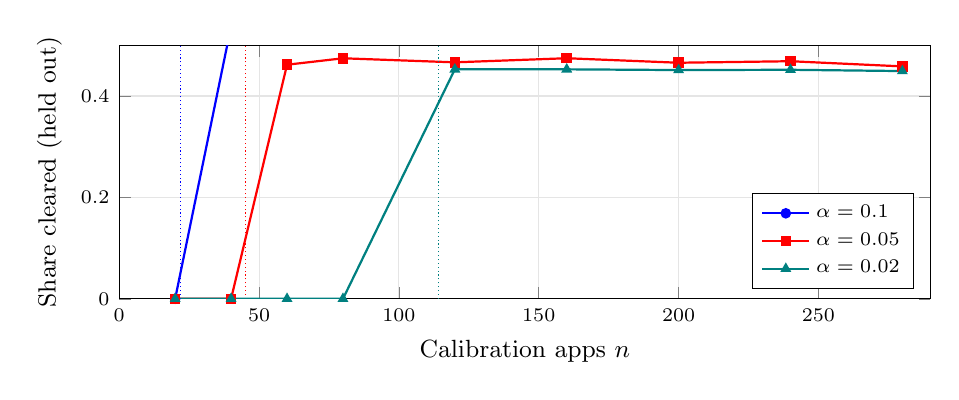
\begin{tikzpicture}
\begin{axis}[width=0.98\linewidth, height=4.8cm, xmin=0, xmax=290, ymin=0, ymax=0.5,
  xlabel={Calibration apps $n$}, ylabel={Share cleared (held out)},
  legend style={font=\scriptsize, at={(0.98,0.04)}, anchor=south east}, legend cell align=left,
  tick label style={font=\scriptsize}, label style={font=\small}, grid=major, grid style={gray!20}]
\addplot[blue, thick, mark=*, mark size=1.5pt] coordinates {(20,0.0000) (40,0.5376) (60,0.5365) (80,0.5642) (120,0.5837) (160,0.5824) (200,0.5952) (240,0.5963) (280,0.6015)};
\addlegendentry{$\alpha=0.1$}
\addplot[blue, densely dotted, thin, forget plot] coordinates {(22,0) (22,0.5)};
\addplot[red, thick, mark=square*, mark size=1.5pt] coordinates {(20,0.0000) (40,0.0000) (60,0.4618) (80,0.4745) (120,0.4665) (160,0.4746) (200,0.4657) (240,0.4687) (280,0.4585)};
\addlegendentry{$\alpha=0.05$}
\addplot[red, densely dotted, thin, forget plot] coordinates {(45,0) (45,0.5)};
\addplot[teal, thick, mark=triangle*, mark size=1.5pt] coordinates {(20,0.0000) (40,0.0000) (60,0.0000) (80,0.0000) (120,0.4527) (160,0.4527) (200,0.4513) (240,0.4518) (280,0.4493)};
\addlegendentry{$\alpha=0.02$}
\addplot[teal, densely dotted, thin, forget plot] coordinates {(114,0) (114,0.5)};
\end{axis}
\end{tikzpicture}

\caption{Certified clearance (Jev, main key) against the number of calibration apps, tested on the remaining apps (mean of 200 draws). Dotted lines: the smallest $n$ at which the exact test can certify each $\alpha$.}
\label{fig:learning}
\end{figure}

\subsection{RQ8: Which design choices matter?}
\label{sec:rq8}
\paragraph{How prices combine.}
With the same cuts and the same calibration, the sum over cut edges clears 40.0\%, the sum over distinct facts 43.0\%, the largest single price 46.8\%, and the independence product 45.3\%, all with at most 1.9\% of held-out apps wrong.
Validity comes from the calibration, not from the union bound; the union bound buys an interpretation, and counting each fact once is valid and free.
\paragraph{Question wording.}
Stating the flow rule in the pricer's question lifted clearance on the first corpus from 15.9\% to 41.1\% at $\alpha=0.10$.
\tabph{3.6cm}{tab:wording}{Question wording: Jev with three wordings.}{Rows: ``taint'' (no-answer type), ``choice'', ``choice with the object convention''; columns: AUROC/ECE on FlowDroid-modeled atoms, main key at $\alpha{=}0.05/0.10$. Source: \texttt{bench/queues/panel\_*.sh} (\textbf{scheduled}).}

\subsection{RQ9: Does the pricer hold up on code it knows less well?}
\label{sec:rq9}
\tabph{4.4cm}{tab:thirdparty}{Pricer quality on third-party libraries (less likely memorized).}{StubDroid summaries generated for OkHttp, Gson, Guava, Commons-Lang/IO, Jsoup, Retrofit; columns: AUROC, ECE, share priced below 0.05 that are real, per library and per pricer. \textbf{Missing}: build the question set (about 1{,}500 questions) with the K2 machinery and price it with Jev and the panel.}

\subsection{RQ10: Does it matter for real leaks?}
\label{sec:rq10}
\tabph{4.4cm}{tab:taintbench}{Documented leaks through library code in a real-malware benchmark.}{TaintBench apps with documented flows: how many documented flows our analysis finds with holes closed and open, how many pass through unmodeled library methods, the receipt price of those that need holes, and what FlowDroid finds. \textbf{Missing}: download the benchmark, run extraction and analysis.}
